
\subsection{Op basis van anonimisatie}

\subsubsection{Agent-Based aanpak door Cissée en Albayrak \cite{CisseeAAP}}

Deze werkwijze spitst zich toe op een Information Filtering (IF) systeem.

Het IF systeem wordt opgesplitst in drie entiteiten: de user, de provider en de filter entiteit. De entiteiten worden in de praktijk door agents vertegenwoordigd. In tegenstelling tot sommige applicaties, waar de provider en de filter door dezelfde partij worden vertegenwoordigd, is dit bij deze werkwijze niet vereist. Dit zorgt voor een meer generieke oplossing. 

Het systeem houdt per entiteit rekening met het respectievelijk privacy aspect. Informatie die mogelijks gelinkt kan worden aan een gebruiker kan niet permanent opgevraagd worden door andere entiteiten. De enige informatie die de provider permanent prijsgeeft zijn de aanbevelingen zelf. Het filteralgoritme kan niet door externe bronnen geraadpleegd worden. Private data van de entiteiten (uitgezonderd de aanbevelingen) wordt enkel tijdelijk beschikbaar gemaakt voor een andere entiteit. Dit wordt mogelijk gemaakt doordat bepaalde entiteiten de communicatie van andere entiteiten kunnen controleren.

Het basisidee is dat de user en provider entiteiten hun data sturen naar de filter entiteit.  De gebruikersdata bestaat uit zijn ratings. De data van de provider bestaat uit een enorme hoeveelheid items, enkel relevante items worden naar de filter gestuurd. Deze filter entiteit berekent de aanbevelingen en verwijdert private data van beide entiteiten. De communicatie tussen de filter entiteit en de user en provider entiteiten gebeurt via een relay entiteit. Die zorgt ervoor dat de zoekopdrachten naar de provider anoniem gebeuren en dus niet gelinkt kunnen worden aan de filterentiteit die tijdelijk de persoonlijke data bevat.

\begin{figure}[htpb]   
    \label{Figuur::anon}      
  \begin{center}    
 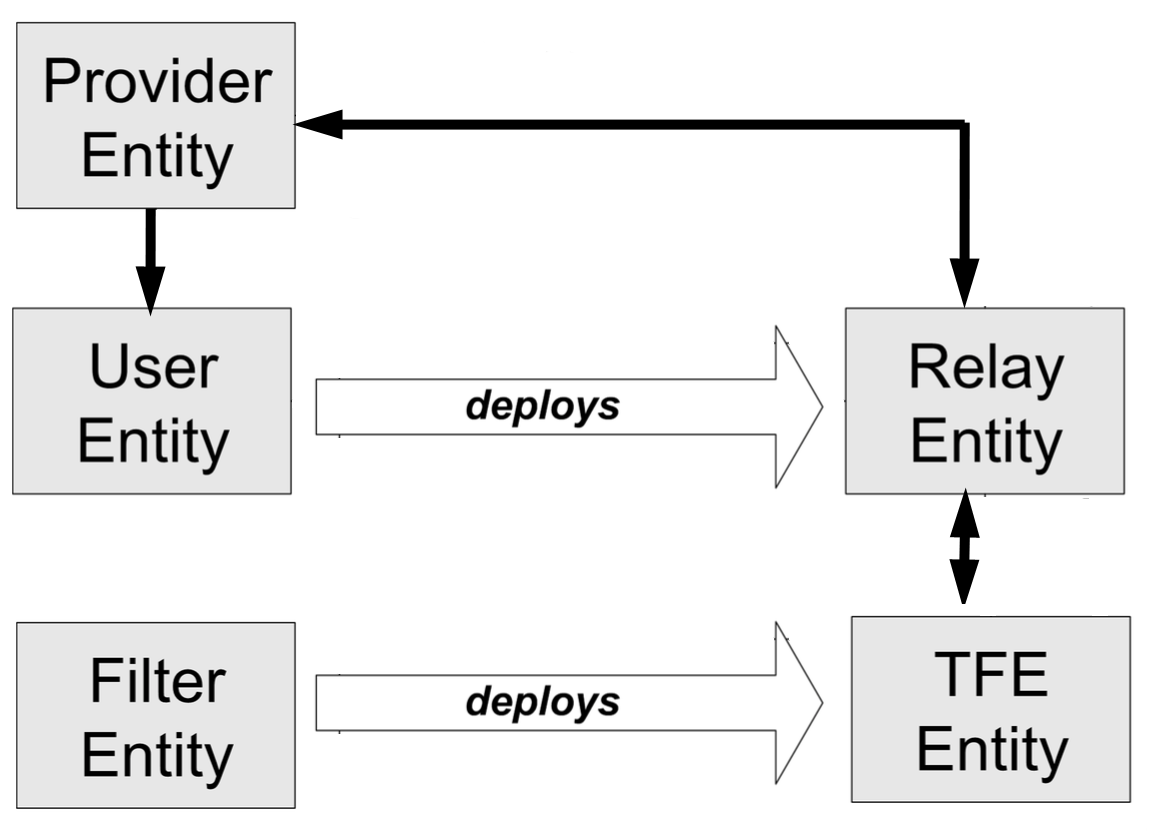
\includegraphics[scale=0.25]{fig/anon}    
  \end{center}   
  \caption{De communicatie tussen de entiteiten, naar \cite{CisseeAAP}. De TFE of \emph{Temporary Filter Entity} handelt de communicatie af voor de filterentiteit.}  
   \end{figure}

In dit artikel kan de op agents gebaseerde aanpak enkel gebruikt worden voor content-based filtering of knowledge-based filtering. Om ook user-user collaborative filtering toe te laten kan  een match-maker module ge\"integreerd worden, beschreven in \cite{CisseeThesis2009}. Hier heeft de provider entiteit de extra taak om de gelijkenissen tussen gebruikers te bepalen. De privacy van de gebruiker wil men garanderen door met pseudoniemen te werken aan de kant van de provider en anonieme communicatie van de provider naar de user toe.\\\\
Belangrijke kenmerken : 
\begin{itemize}


\item Berekeningen van de aanbevelingen gebeuren in de vertrouwde filter entiteit.
\end{itemize}
Voordelen : 
\begin{itemize}


\item Houdt ook rekening met de privacy van de provider en het gebruikte algoritme.

\end{itemize}
Nadelen:
\begin{itemize}
\item Anonimisatie van de zoekopdrachten door middel van relay entiteiten bij het kennis-gebaseerde aanbevelingssysteem zou kunnen leiden tot re\"identificatie van de gebruikers. Dit kan ook het geval zijn bij het gebruik van pseudoniemen in het user-user collaborative filtering systeem.
\item De filter agent moet worden vertrouwd door de gebruiker en mag niet samenvallen met de provider.
\item Het aanmaken van agents en bijhorende communicatieplatformen cre\" eert extra overhead wat de performantie benadeelt. Een aanbeveling met dit systeem duurt ongeveer 10 maal zo lang als een normale aanbeveling.

\end{itemize}